% Block diagram of the autonomous driving software (Section 2.4).
\begin{tikzpicture}[
    font=\footnotesize,
    >={Stealth[length=2mm]},
    blk/.style={draw, rounded corners=2pt, align=center, minimum height=8mm, inner sep=3pt},
    sens/.style={blk, minimum width=17mm, fill=gray!8},
    mod/.style={blk, minimum width=21mm, fill=blue!6},
    hl/.style={blk, minimum width=21mm, fill=blue!18, very thick},
    grp/.style={draw, dashed, rounded corners=4pt, inner sep=5pt},
    lab/.style={font=\scriptsize, align=center, text=black!70},
    line/.style={->, thick}
]
% sensors
\node[sens] (lidar) {LiDAR};
\node[sens, below=2mm of lidar] (radar) {RaDAR};
\node[sens, below=2mm of radar] (cam) {Camera};

% perception
\node[mod, right=12mm of radar, minimum height=25mm] (det) {Detection\\(per sensor)};
\node[hl, right=14mm of det] (trk) {Target\\tracking};
\node[grp, fit=(det)(trk), label={[lab]above:Perception}] (P) {};

% localization, below perception; GNSS/INS at the same height
\node[mod, below=10mm of P.south, anchor=north] (loc) {Localization};
\node[sens] (gnss) at (cam |- loc) {GNSS / INS};
\node[grp, fit=(lidar)(radar)(cam)(gnss), label={[lab]above:Sensors}] (S) {};

% planning, control, actuators
\node[mod, right=18mm of trk] (plan) {Planning};
\node[mod, fill=gray!8, above=9mm of plan] (db) {Track\\database};
\node[mod] (ctrl) at (plan |- loc) {Control};
\node[sens, below=9mm of ctrl] (act) {Actuators};

% data flow
\foreach \s in {lidar,radar,cam} \draw[line] (\s.east) -- (\s.east -| det.west);
\draw[line] (det) -- node[lab, above]{detections} (trk);
\draw[line] (gnss) -- (loc);
\draw[line] (loc) -- node[lab, right]{ego state} (loc |- P.south);
\draw[line] ([yshift=1.5mm]trk.east) -- node[lab, above]{opponents} ([yshift=1.5mm]plan.west);
\draw[line] (db) -- (plan);
\draw[line] (plan) -- node[lab, right]{reference\\trajectory} (ctrl);
\coordinate (bus) at ($(trk.east)!0.5!(plan.west)$);
\draw[line] (loc) -- node[lab, below, pos=0.35]{ego state} (ctrl);
\draw[line] (bus |- loc) |- ([yshift=-2mm]plan.west);
\fill (bus |- loc) circle (0.8pt);
\draw[line] (ctrl) -- node[lab, right]{steering, throttle,\\brake, gear} (act);

% vehicle, closing the loop between actuators and sensors
\node[inner sep=1pt, label={[lab]below:Vehicle}] (car) at (loc |- act) {\reflectbox{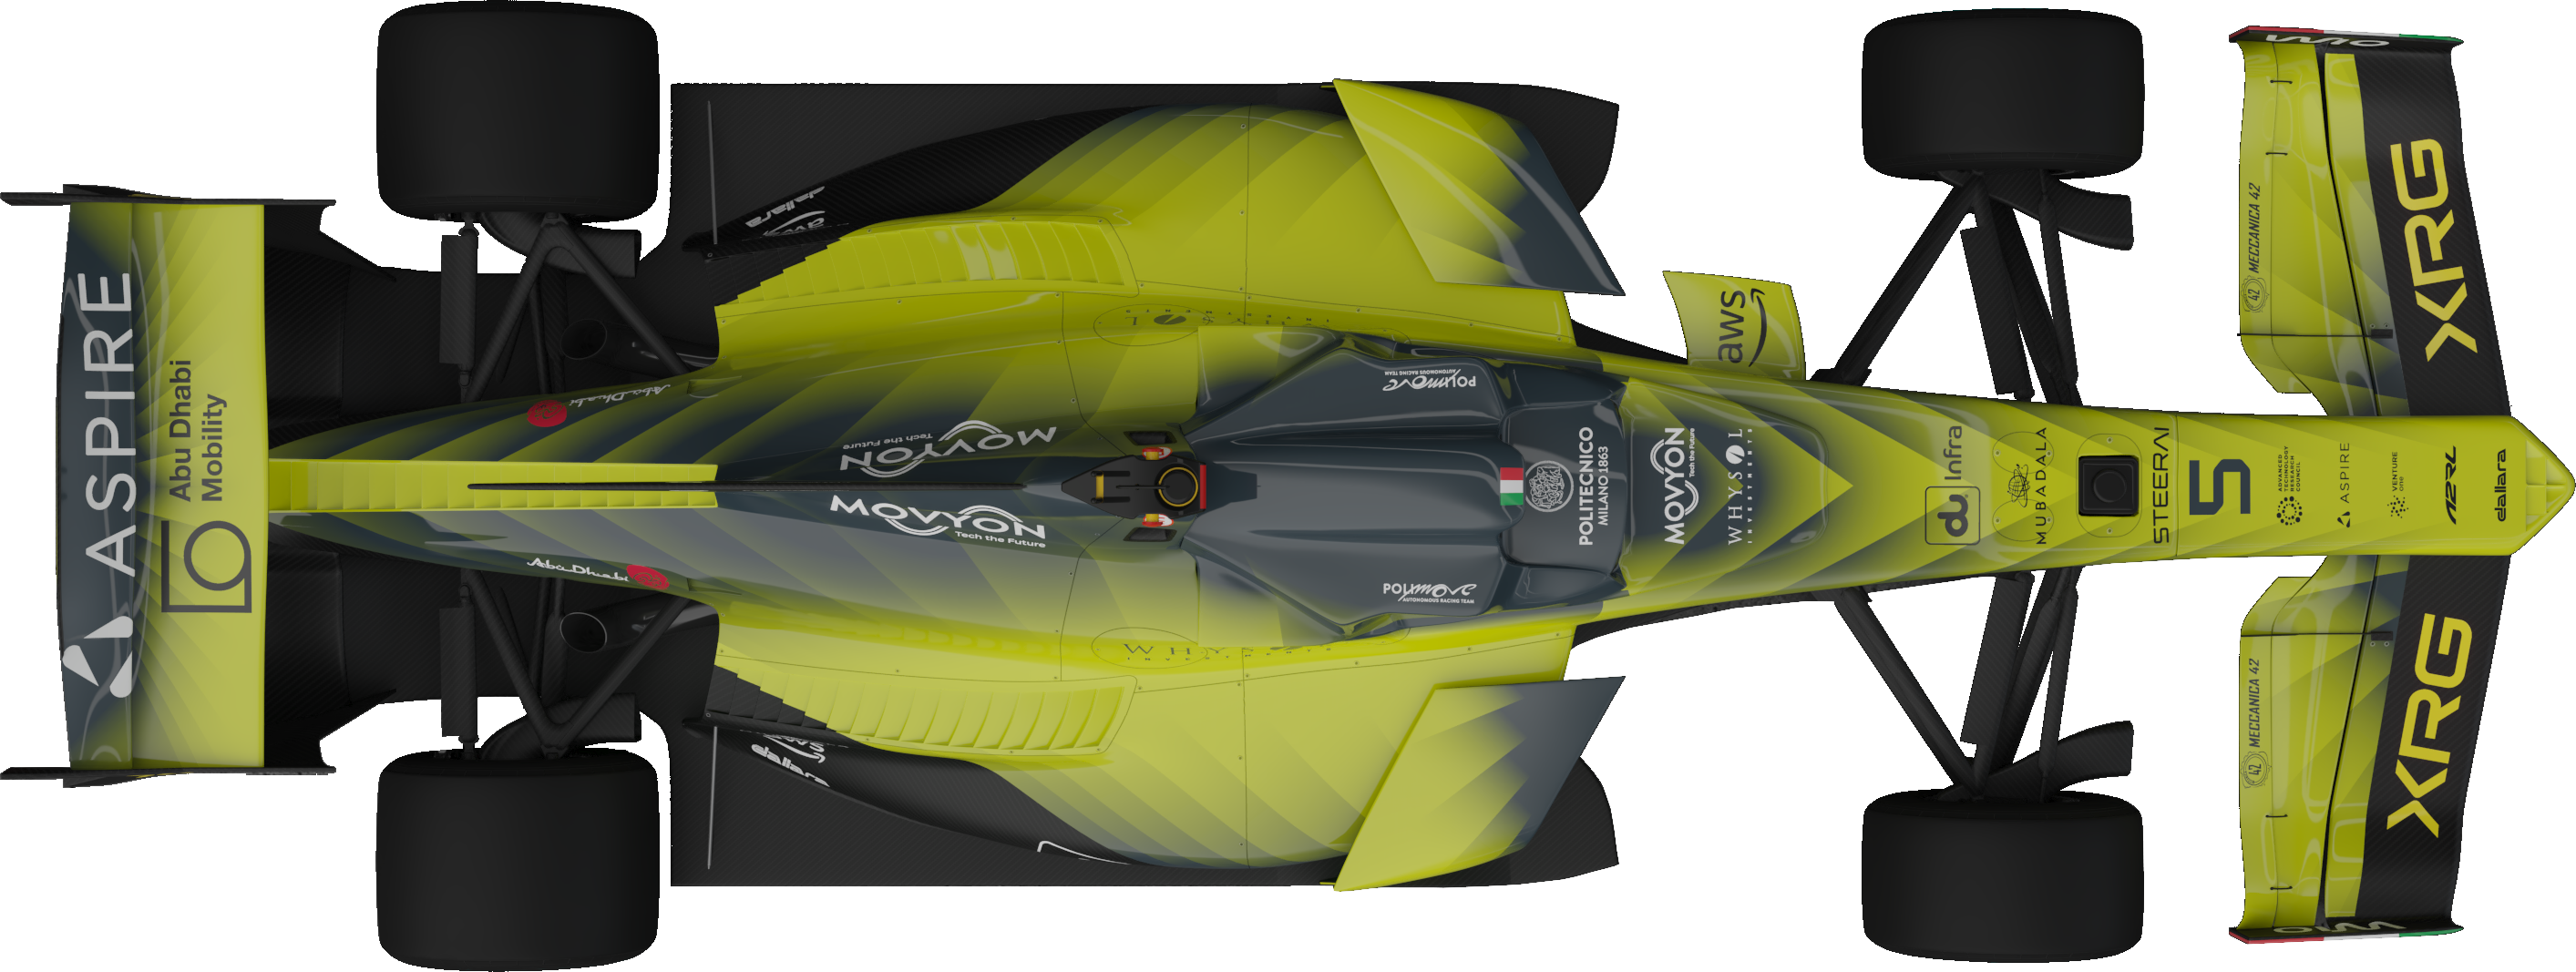
\includegraphics[width=30mm]{figures/ch2/src/eav24_top.png}}};
\draw[line] (act) -- (car);
\draw[line] (car) -| (S.south);
\end{tikzpicture}
